
\section{Introduction}
   
        Forecasting the behavior of a large-scale real-world system directly from first principles often requires solving highly-nonlinear governing equations such as high-dimensional ordinary differential equations (ODEs) or partial differential equations (PDEs). 
        High-fidelity simulations of such dynamical systems can become intractable especially if an online control algorithm requires multiple forecasts per second using a low-powered embedded device \cite{rowley2017model,lucia2004reduced,benner2015survey}. A situation like this arises, for example, when a smart heating, ventilation, and air conditioning (HVAC) system attempts to optimize the temperature distribution of the air in a room using only partial measurements \cite{farahmand2016learning,nabi2022robust}. At the moment of writing this paper such systems are incapable of real-time complex simulations, but they already can run low-dimensional pre-trained models, thus inviting the development of high-quality reduced order models (ROMs) \cite{otterness2017evaluation} . ROMs, therefore, are essential for enabling design optimization, uncertainty propagation, predictive models, and control for such dynamical systems \cite{brunton2022data,kutz2016dynamic,rowley2017model,jones2020characterising}
        
        To be suitable for control, a ROM training method needs to find a low-dimensional manifold and a dynamics on it that together yield both high-accuracy predictions and long-term stability \cite{ahmed2021closures,noack2011reduced}. Most traditional ROMs are projection-based, e.g. dynamic mode decomposition (DMD) \cite{kutz2016dynamic,tu2013dynamic} and proper orthogonal decomposition (POD) \cite{holmes2012turbulence}, which transform the trajectories of a high-dimensional dynamical system into a suitable, and in some sense optimal, low-dimensional subspace. This projection leads to truncation of higher order modes and parametric uncertainties, which result in large prediction errors over time due to the deterioration of basis functions (spatial modes) \cite{benner2015survey}. 
        One challenge for POD methods is their intrusive nature, i.e. requiring access to the solver codes.
       To overcome this, operator inference approaches \cite{qian2020lift,peherstorfer2016data} utilize SVD-based model reduction and then exploit lifting to fit the latent space dynamics data into
        polynomial, typically quadratic, models.
        These models, however, are (i) limited in representation power (up to quadratic, e.g. for lift and learn approach) and (ii) require a custom-tailored SVD-based optimization technique. 
        
        
        In a thrust to overcome these challenges, significant effort has been invested into developing autoencoder-based reduced-order models, as a popular nonlinear ROM technique, which can yield both accurate and stable ROMs \cite{lee2020model,gin2021deep,champion2019data,kim2019deep}. In practice, however, they require datasets that densely cover a hypothetical infinite dimensional phase portrait of the dynamical system. Large demand for data significantly limits the use of such models in physics applications where the data can be expensive to obtain.
    

        Another severe challenge of utilizing ROMs comes from their poor out-of-distribution performance \cite{fries2022lasdi,cranmer2020discovering,gin2021deep}, especially when it is fundamentally impossible for a practitioner to obtain data that covers the entire distribution of possible data inputs. For example, in HVAC applications, one may collect data from a room with two windows but not from one room for every possible number of windows. In atmospheric LiDAR applications, we may conduct experiments on a certain terrain but we can never conduct experiments on all sorts of terrains \cite{nabi2020improving}. In such situations embedding the knowledge of physics into a model becomes necessary to improve extrapolation performance, and for which several approaches have recently been proposed.
        For instance, the seminal works \cite{bongard2007automated,schmidt2009distilling} have tried to determine the underlying structure of a nonlinear dynamical system from data using symbolic regression. Recently, Cranmer et al. \cite{cranmer2020discovering} employed symbolic regression in conjunction with graph neural network (GNN), while encouraging sparse latent representation, to extract explicit physical relations. They showed that the symbolic expressions extracted from the GNN generalized to out-of-distribution- data better than the GNN itself. However, symbolic regression also suffers from excessive computational costs,  and may be prone to overfitting.

      

        Another example of incorporating physics in ROMs is the use of parametric models at the latent space, e.g. by using the sparse identification of nonlinear dynamics (SINDy) \cite{brunton2016discovering,champion2019data}. For instance, \cite{fries2022lasdi,he2022glasdi} used a chain-rule based loss that ties latent-space derivatives to the observable-space derivatives for simultaneous training of the auto-encoder and the latent dynamics. However, such loss is highly sensitive to noise in data, especially when evaluating time-derivatives with finite differences is required\cite{delahunt2022sindynoise}. 
        Collocation-based enforcement of the physics, i.e. projection of the candid functions in the governing equations to enforce the chain rule instead of finite difference, could address such numerical difficulties. Recently, Liu et al. \cite{liu2022physics} used auto-encoder architecture and Koopman theory to demonstrate that combining autoencoders with enforcing linear dynamics in the latent space may result in an interpretable ROM. However, linearity may not be expressive enough for complex dynamics with multiple basins of attraction \cite{page2019koopman}.
        Finally, recent works on NeuralODE (NODE) \cite{chen2018neuralode,rackauckas2020udes} show a way to fit an arbitrary non-linear model (e.g. a network) as a latent space dynamics model, significantly extending the set of models for the latent dynamics that one can train efficiently. 
        
        In this paper, we employ autoencoders to perform nonlinear model reduction along with NODE at the latent space to model complex and nonlinear dynamics. Our goal is to reduce their demand for data and improve overall forecasting stability under challenging training conditions. To achieve that we build on ideas from classical collocation methods of numerical analysis to embed knowledge from a known governing equation into the latent-space dynamics of a ROM, as described in Section 2. Then, in Section 3, we show that addition of our physics-informed loss allows for exceptional data supply strategies that improves the performance of ROMs in data-scarce settings, where training high-quality data-driven models is impossible. We demonstrate that such an approach not only reduces the need for large training data-sets and produces highly-accurate and long-term stable models, but also leads to the discovery of more compact latent spaces, which is especially important for applications in compressed sensing and control.

       
            \begin{figure}[t]
    \centering
    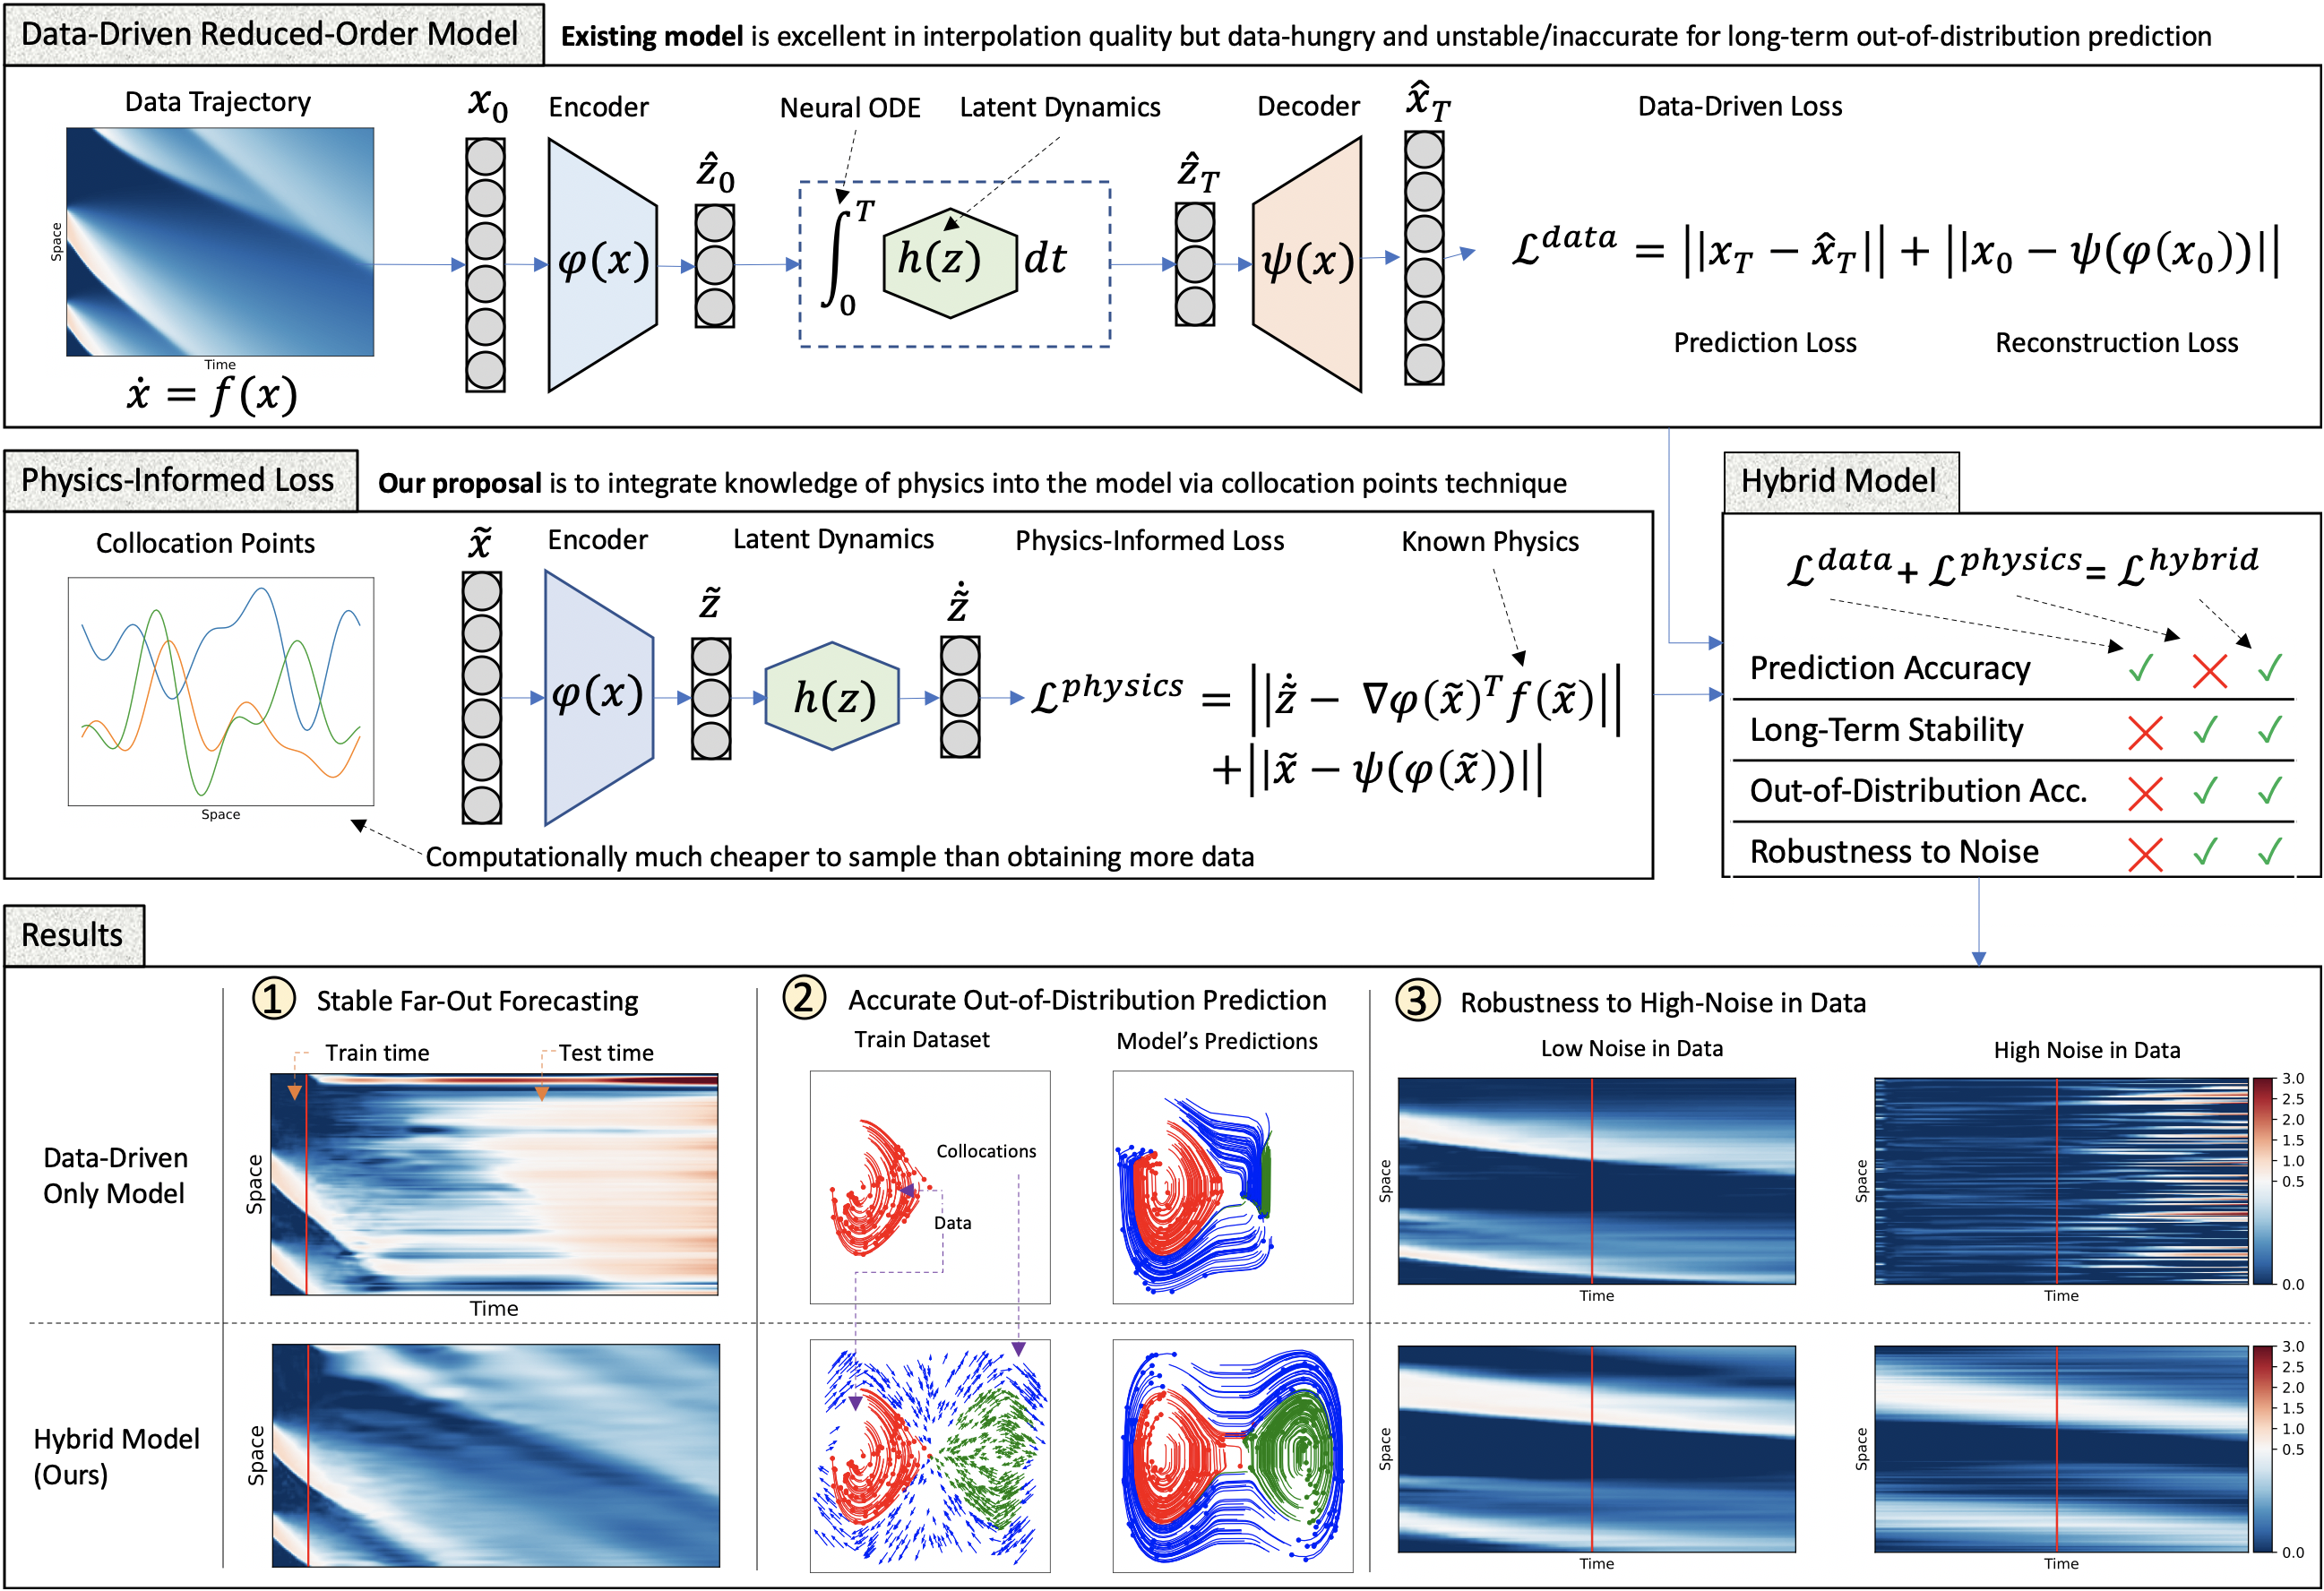
\includegraphics[width=\textwidth]{figures/graphical-abstract.png}
    \caption{We propose utilizing a collocation points technique from numerical analysis to transfer knowledge of physics into continuous-time reduced-order models (ROMs). Such physics-informed models yield orders of magnitude more accurate predictions in tasks of far-out forecasting, predictions for out-of-distribution initial conditions, and learning from high-noise data. Good performance on those tasks is crucial for using ROMs in problems of compressive sensing and control.}
    \label{fig:architecture}
\end{figure}

\section{Method}
\label{sec:method}
\paragraph{Reduced-Order Model with Non-Linear Latent Dynamics}
We consider an autonomous dynamical system on a finite space $\XX \subseteq \mathbb{R}^n$

\begin{equation}
    \label{eq:generic_stationary_ode}
        \ddt\bd{x}(t) = \bd{f}(\bd{x}(t))
\end{equation}

In real-world applications it is often expensive to solve the relationship~(\ref{eq:generic_stationary_ode}) directly because $x(t)$ can be very high-dimensional. However, a variety of works provided both theoretical \cite{holmes2012turbulence} and practical \cite{noack2011reduced,chen2021discovering} evidence that many physical systems evolve on a manifold $\ZZ \subseteq \mathbb{R}^m$ of a lower dimension $m << n$. In that space, the dynamics evolve according to a (generally unknown) function  $\bd{h}(\bd{z})$:

\begin{equation}
    \label{eq:latent_stationary_ode}
        \ddt\bd{z}(t) = \bd{h}(\bd{z}(t))
\end{equation}

We call the space $\XX$ an observable space, and $\ZZ$ a latent space. When an invertible mapping $\psi:\ \ZZ \to \XX$ between the observable and the latent spaces is known, one can predict the dynamics of the system $\bd{x}$ at a future time $T$ by projecting the initial condition $\bd{x}(0)$ into the latent space, performing an integration there, and mapping the resulting trajectory back to the observable space:
\begin{equation}
\label{eq:integration_in_latent_space}
\begin{split}
    \bd{z}(0) & = \psi^{-1}(\bd{x}(0)) \\
    \bd{z}(T) & = \bd{z}(0) + \int_{0}^T\bd{h}(\bd{z}(t))dt \\
    \bd{x}(T) & = \psi(\bd{z}(T))
\end{split}
\end{equation}

When $m << n$ we refer to the triplet $(\psi, \psi^{-1}, \bd{h})$ as a Reduced-Order Model (ROM) of $\bd{f}$. It is often the case that for a given system $\bd{f}$ there exists no ROM $(\psi, \psi^{-1}, \bd{h})$ such that the relation~(\ref{eq:integration_in_latent_space}) holds exactly. In this case, we seek an \textit{approximation} ROM $(\psi_{\theta^*}, \phi_{\theta^*}, h_{\theta^*})$ that minimizes the difference between the data $x(t)$ and the prediction $\hat{x}(t)$ over a chosen class of models $(\psi_\theta, \phi_\theta, h_\theta)$ parameterized by $\theta$.

Multiple real-world applications necessitate using ROMs instead of integrating the relation~(\ref{eq:generic_stationary_ode}) directly. For example, integrating~(\ref{eq:generic_stationary_ode}) may be computationally intractable especially on platforms with limited computing capability such as embedded and autonomous devices. For instance, in an HVAC system, solving~(\ref{eq:generic_stationary_ode}) means solving a Navier-Stocks equation on a fine grid in real time, which exceeds the computing capabilities of current-generation appliances. On the other hand, integrating~(\ref{eq:integration_in_latent_space}) may be cheap when $m << n$. Finally, even when solving~(\ref{eq:generic_stationary_ode}) is possible in real time (e.g. by utilizing a remote cluster), executing control over the resulting model, which is an end-goal for an HVAC system, may still be intractable. Indeed, executing control requires \textit{multiple} iterative evaluations of~(\ref{eq:generic_stationary_ode}) for \textit{each} iteration of control even for the most efficient algorithms known to date~\cite{duriez2017machine}. 

\paragraph{Architecture} In this work we model $\psi$, $\psi^{-1}$, and $\bd{h}$ with fully-connected neural networks $\psi_\theta$, $\phi_\theta$, and $h_\theta$, respectively. Specifically, the pair ($\psi$, $\psi^{-1}$) is modelled with an auto-encoder $(\psi_\theta, \phi_\theta)$, and $\bd{h}$ is modelled with a fully-connected network $h_\theta$. Figure~\ref{fig:architecture} visualizes the architecture of the model. 

\paragraph{Data-Driven Loss} Similar to prior works \cite{takeishi2017learning,morton2019deep,gin2021deep}, we define a \textit{data-driven loss} $\LL_{data}$ as a sum of reconstruction and prediction losses. The former ensures that $\phi_\theta$ and $\psi_\theta$ are inverse mappings of each other, whereas the latter matches the model's predictions to the available data. Formally, for a given set of trajectories $\bd{x}_i$, $i \in [1 \dots k]$, where each trajectory $\bd{x}_i \in \mathbb{R}^{n \times p}$ is a set of $p$ snapshots that correspond to the recorded states of the system for $p$ time-steps, $t_j$, $j \in [1, \dots, p]$, the loss function $\LL^{data}_\theta$ is defined as:

\begin{align}
    \label{eq:loss_data_driven}
    \LL^{data}_\theta & = \frac{1}{2\sigma^2}\sum_{i = 1}^k \left[\frac{\omega_1}{p}\sum_{j=1}^p\left\|\bd{x_i}(t_j) - \psi_\theta(\phi_\theta(\bd{x_i}(t_j)))\right\|^2\right. + \\
     & + \left.\frac{\omega_2}{p}\sum_{j=1}^p \left\|\psi_\theta\left(\phi_\theta(\bd{x_i}(t_1)) + \int_{t_1}^{t_j}h(z(t))dt\right) - \bd{x_i}(t_j)\right\|^2 \right]
\end{align}
where $\sigma$ is the standard deviation of the observation noise. We note that each trajectory $\bd{x}_i$ may be captured over its own time-frame and use a distinct, possibly non-uniform, step-size, in which case the loss function should be modified accordingly\footnote{The implementation is affected only in evaluating the integral in~(\ref{eq:loss_data_driven}). This part is handled by \texttt{torchdiffeq}~\cite{chen2018neural} library, which supports non-uniform time-frames within a batch}. To simplify the notation without loss of generality, in the rest of the paper we assume that all trajectories were recorded over the same time-frame with an equal and uniform step-size. 

\paragraph{Physics-Informed Loss} In their recent work, \cite{liu2022physics} proposed a method for utilizing knowledge of the governing equations $d\bd{x}/dt = \bd{f(x)}$ as a finite-dimensional approximation of Koopman eigenfunctions for linear latent dynamics. To extend this approach to the non-linear regime, we note that for a true mapping $\phi$ the following holds:
\begin{equation}
    \label{eq:chain_rule_1}
    \frac{d\bd{z}(\bd{x}(t))}{dt} = \frac{d\bd{z}}{d\bd{x}}\frac{d\bd{x}}{dt} = \nabla\phi(\bd{x}(t))^T\bf{f}(\bd{x(t)})
\end{equation}
On the other hand, by the definition of $\psi$ and $\bd{h}$ we have that
\begin{equation}
    \label{eq:chain_rule_2}
    \frac{d\bd{z}(\bd{x}(t))}{dt} = \bd{h}(\phi(\bd{x}(t))
\end{equation}
Combining Equations~(\ref{eq:chain_rule_1}) and~(\ref{eq:chain_rule_2}) we get that
\begin{equation}
    \label{eq:physsics_informed_equation}
    \bd{h}(\phi(\bd{x}(t)) = \nabla\phi(\bd{x})^T\bd{f}(\bd{x})
\end{equation}
Equation~(\ref{eq:physsics_informed_equation}) links the dynamics $\bd{h}(\bd{z})$ and the encoder $\phi(\bd{x})$ with the known equation $\bd{f}(\bd{x})$ and is true for all $z \in \ZZ$ and $x \in \XX$. Hence, knowledge of $\bd{f}$ can be assimilated into the model by evaluating Equation~(\ref{eq:physsics_informed_equation}) on a set of $N$ carefully sampled points $\bar{\bd{x}}_i \in \XX$, $i \in [1, \dots, N]$:

\begin{equation}
    \label{eq:loss_physics_informed}
    \LL^{physics}_\theta = \sum_{i = 1}^N \left[\frac{\omega_3}{N}\left\|h_\theta(\phi_\theta(\bar{\bd{x}}_i)) - \nabla \phi_\theta(\bar{\bd{x}}_i) \bd{f}(\bar{\bd{x}_i})\right\|^2 + \frac{\omega_4}{N}\left\|\bar{\bd{x}}_i - \psi_\theta(\phi_\theta(\bar{\bd{x}}_i))\right\|\right]
\end{equation}

We refer to the points $\bar{\bd{x}}_i$ as \textit{collocations}.

\paragraph{Collocations}
\label{sec:collocations_conditions} We define a collocation as pair $(\bd{\bar{x}},\, \bd{f}(\bd{\bar{x}}))$. Collocations are samples from the space $\XX \times Im_{f}(\XX)$, and they should satisfy three conditions, ordered by importance:
\begin{enumerate}
    \item \textbf{Simplicity}: $\bd{f}(\bar{\bd{x}}_j)$ should be computationally cheap to evaluate. It is especially important for PDE systems, where $\bd{f}$ may involve high-order derivatives.
    \item \textbf{Representativeness}: $\bar{\bd{x}}_j$ should cover the space of states where one aims to improve the model's performance or stability. Collocation points that a model might encounter and that are not represented by data snapshots are the best candidates.
    \item \textbf{Feasibility}: $\bar{\bd{x}}_j \in \XX$. In other words, $x_j$ should be an attainable state of the system. Collocation points outside of $\XX$ may downgrade the performance of the autoencoder by forcing it to be an invertible function on a domain outside of $\XX$ where a true mapping $\psi$ operates on.
\end{enumerate}
Thus, an optimal sampling procedure for collocations $\bd{\bar{x}}_j$ is domain-specific and should be designed given a particular system $\bd{f}$ and available data $\bd{x}_i$. We show examples of how these conditions can be implemented for real systems in the following sections.

Our definition of collocation points follows recent works\cite{liu2022physics}, which is a further development of the original definition \cite{raissi2018hidden} with the difference being the sample space: instead of sampling from the spatiotemporal domain we sample them from an appropriate function space. 

\paragraph{Combined Loss Function} We train the model by optimizing a sum of the physics-informed loss~(\ref{eq:loss_physics_informed}) and the data-driven loss~(\ref{eq:loss_data_driven}):
\begin{equation}
    \label{eq:loss_combined}
    \min_\theta \left[\LL^{physics}_\theta + \LL^{data}_\theta\right]  
\end{equation}
When $\omega_1 = \omega_2 = 0$ we have that $\LL^{data}_\theta = 0$, so we say that the model is (purely) \textit{\textbf{Physics-Informed}}. Similarly, when $\omega_3 = \omega_4 = 0$ we have that $\LL^{physics}_\theta = 0$ and we say that the model is (purely) \textit{\textbf{Data-Driven}}. When $\omega_i \neq 0, \, \forall i$, we say that the model is \textit{\textbf{Hybrid}}.

We use a \texttt{pytorch}~\cite{NEURIPS2019_9015} implementation of Adam algorithm~\cite{kingma2014adam} for optimization. To evaluate $\nabla_\theta \LL^{physics}_\theta$ and $\nabla_\theta \LL^{data}_\theta$ we use \texttt{torchdiffeq}~\cite{chen2018neural} -- a \texttt{pytorch}-compatible implementation of Neural ODE framework. 

To the best of our knowledge, this is the first framework that combines non-linear latent-dynamics (Neural ODE), autoencoders, and a physics-informed loss term~(\ref{eq:loss_physics_informed}). Thus, we call our framework \textit{Physics-Informed Neural ODE}, or PINODE. 

\section{Experiments}
\label{sec:exp}
The experiments section is organized as follows. First, to illustrate the ideas behind the framework we study its performance on a high-dimensional ODE -- a lifted Duffing oscillator. We show how a non-linear latent dynamics $\bd{h}(\bd{z})$ overcomes the limitations of DMD and Koopman networks from \cite{liu2022physics} by handling multiple basins of attraction within one model. We also show that using physics-informed loss is sufficient for reconstructing the behaviour for basins of attraction that are not represented by the data. Finally, we demonstrate that a purely data-driven model may be highly-accurate short-term and highly unstable long-term, even when the data is abundant, and show that the physics-informed approach improves long-term stability of such models by multiple orders of magnitude.

Next, we study the framework's performance on Burgers' equation. We show that (i) the non-linear latent dynamics yields more compact latent spaces than its linear counterpart for the same accuracy; (ii) these compact latent spaces allow for more stable long-term predictions; (iii) in the presence of significant noise in data, the use of collocations improves stability by providing an extra source of information that is noise-free, and (iv) in certain scenarios, training \textit{only} on collocations yields \textit{better} models than training on data, even when a vast amount of data is available. The latter shows that the contribution of physics-informed loss~(\ref{eq:loss_physics_informed}) may surpass the one of the data-based loss~(\ref{eq:loss_data_driven}), especially when the data is severely limited or noisy. 

\begin{figure}[t]
    \centering
    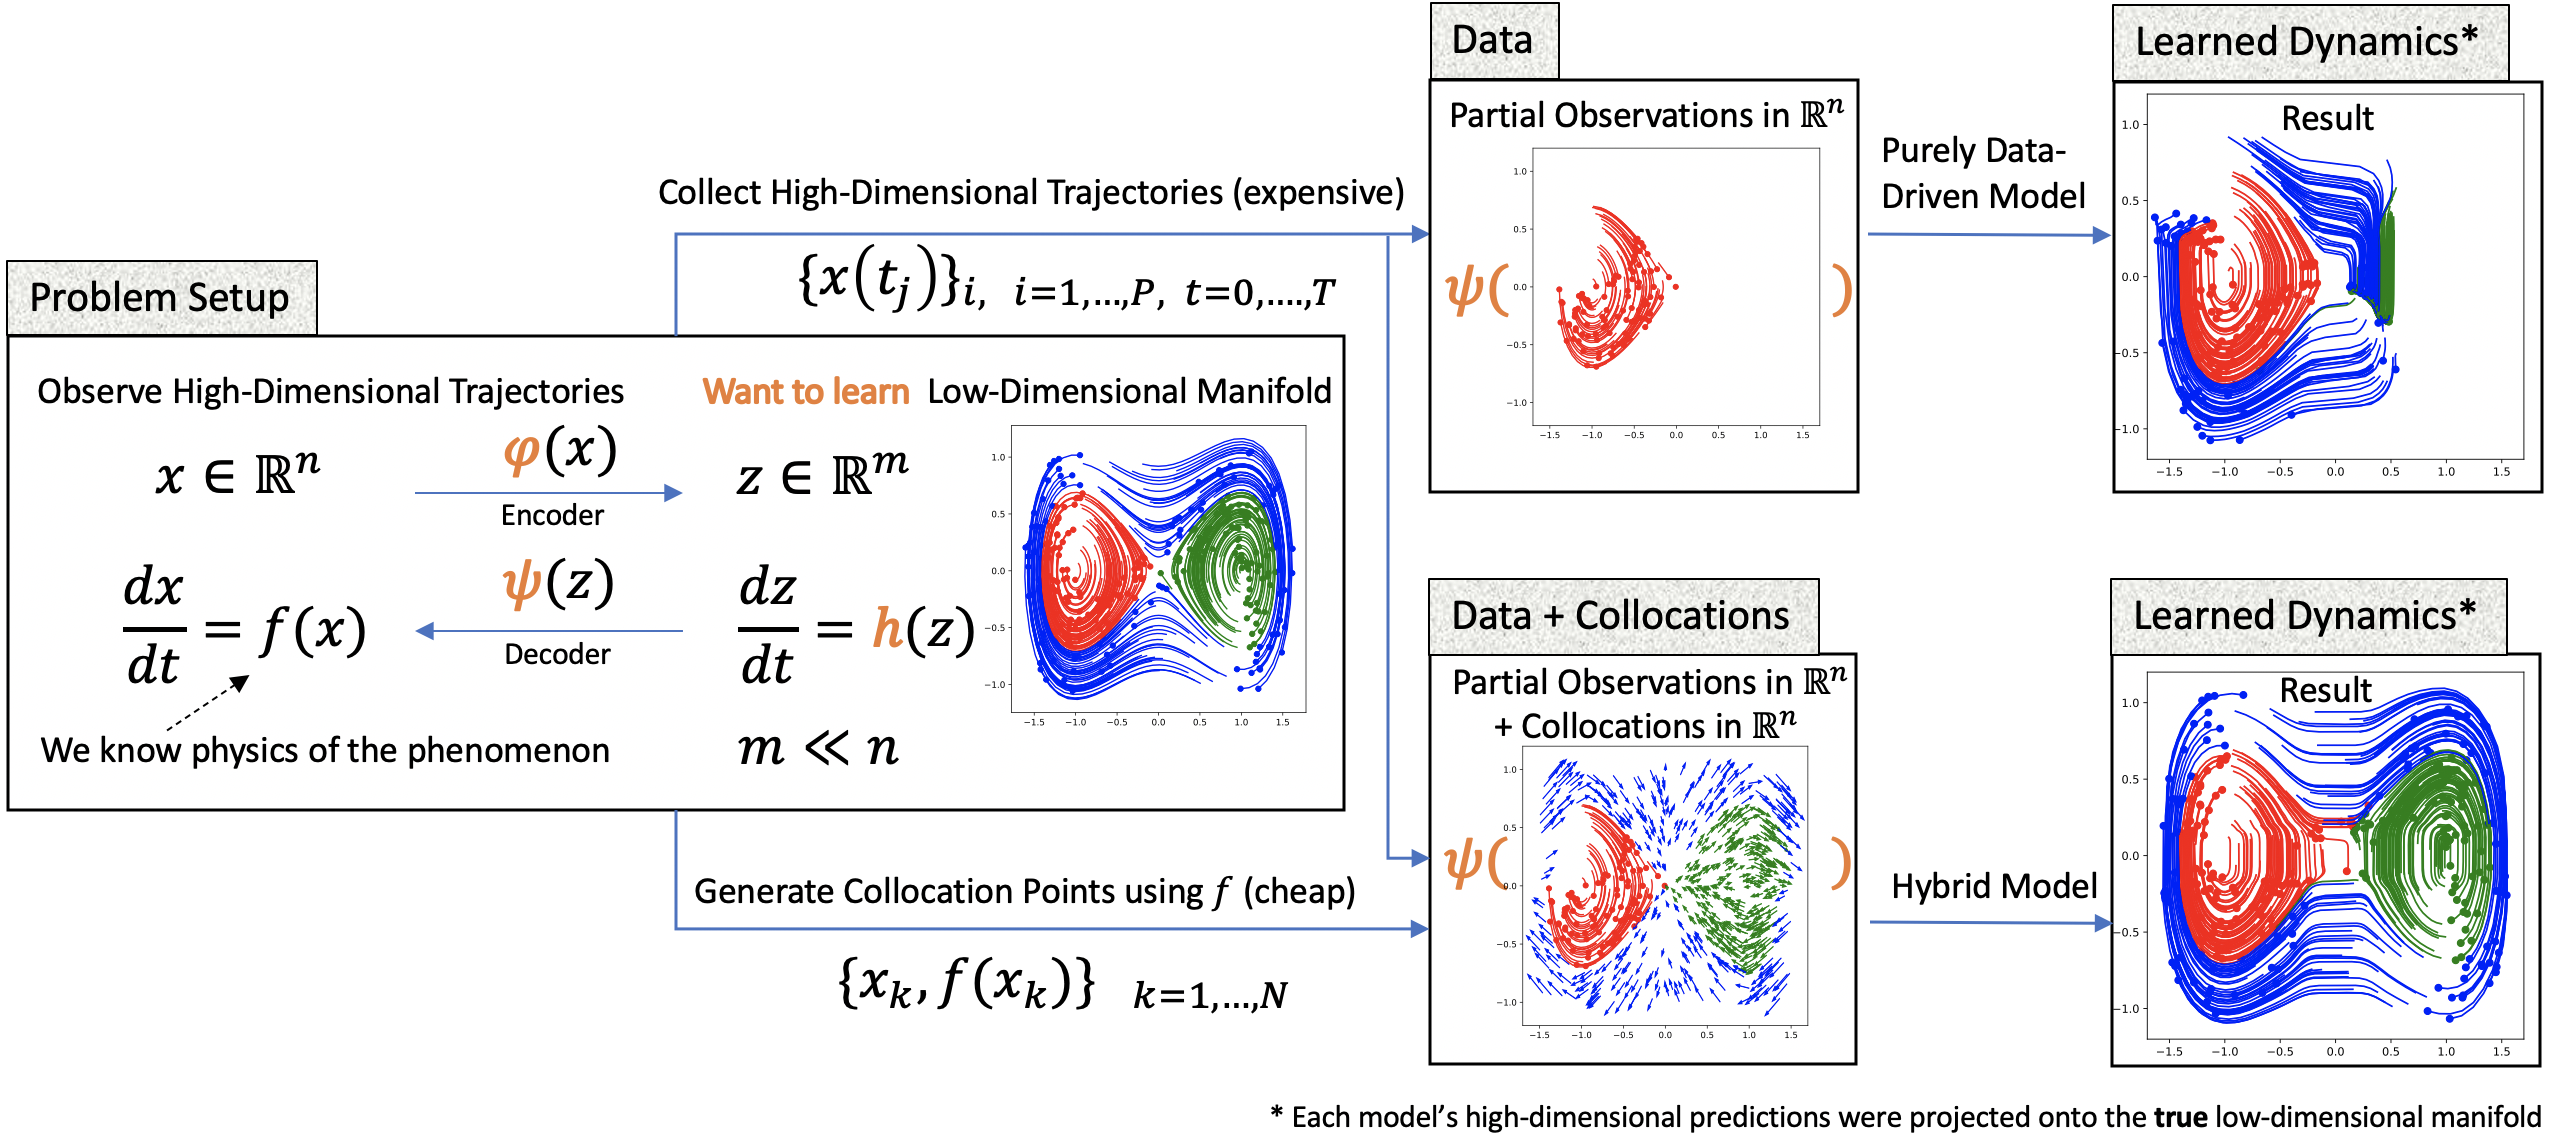
\includegraphics[width=\textwidth]{figures/duff_first_exp_abstract.png}
    \caption{We use a toy example -- a Lifted Duffing Oscillator -- to show that it is possible to ``fill the gaps'' in data with collocations. Namely, Hybrid model from Figure~\ref{fig:architecture} is able to learn the dynamics of two additional basins of attraction that were not represented in the dataset. As shown in the top-rightmost frame, without the collocations the model does not infer the dynamics in the unseen regions correctly.}
    \label{fig:duffing_pinode}
\end{figure}

\newpage
\subsection{Lifted Duffing Oscillator}
\label{sec:duffing}

A Duffing oscillator is a dynamical system $d\bd{z}/dt = \bd{h}(\bd{z})$ such that 

\begin{equation}
    \label{eq:duffing_definition}
    \begin{split}
    \frac{dz_1}{dt} & = z_2 \\ 
    \frac{dz_2}{dt} & = z_1 - z_1^3
    \end{split}
\end{equation}


A phase portrait for 300 randomly sampled trajectories from this system is visualized on Figure~\ref{fig:duffing_pinode}, left frame. Depending on the total energy, each trajectory always stays in one of three regions: the left lobe, the right lobe, or the outer area, visualized in red, green, and blue respectively. To create a synthetic high-dimensional system that retains this property, we lift the Duffing trajectories into a higher-dimensional space by applying an invertible transformation $\mathcal{A}(\bd{z})$: 

\begin{equation}
    \label{eq:duffing_true_decoder}
    \bd{x} := \mathcal{A}(\bd{z}) = A\bd{z}^3, \quad A \in \mathbb{R}^{128 \times 2}, \quad A_{ij} \sim_{i.i.d.} \mathcal{N}(0, 1)
\end{equation}

\begin{wrapfigure}{r}{0.25\textwidth}
  \begin{center}
    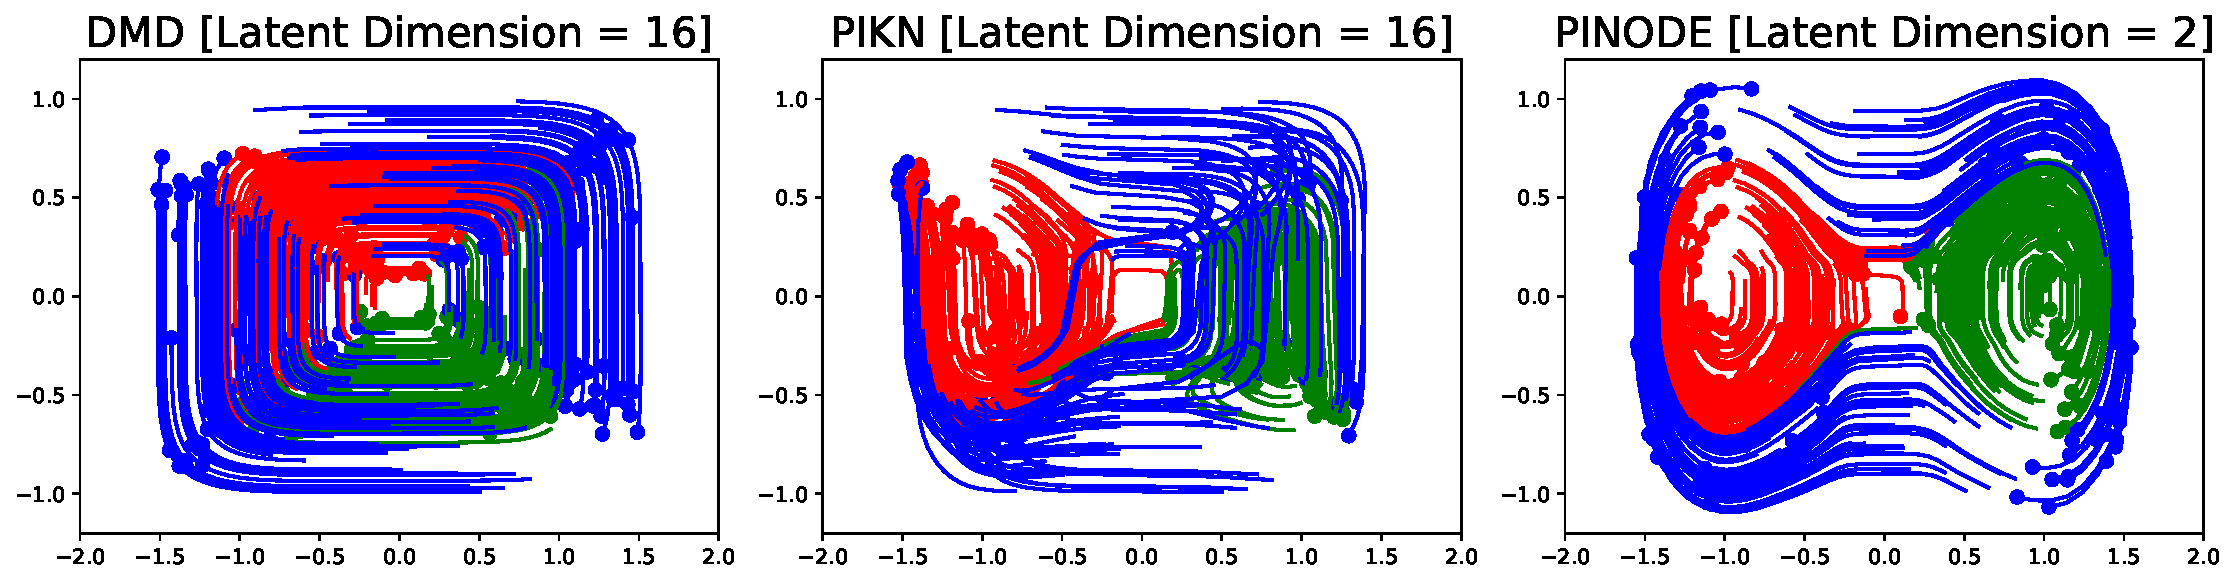
\includegraphics[width=0.23\textwidth]{figures/duffing_comparison.pdf}
  \end{center}
  \caption{Non-linearity in latent dynamics and autoencoder is important for long-term extrapolation. PIKN Hybrid model was unable to extrapolate the dynamics from collocations, while PINODE Hybrid model was.}%\vspace{-0.5in}
  \label{fig:duffing_comparison}
\end{wrapfigure}
Hence, for this system $z \in \ZZ = \mathbb{R}^2$ and $\bd{x} \in \XX = \text{span}\{A_{:,1}, A_{:,2}\} \subseteq \mathbb{R}^{128}$. We treat $\XX$ as an observable space, in which the dynamical system~(\ref{eq:duffing_definition}) obeys the following:
\begin{equation}
    \frac{d\bd{x}}{dt} = \bd{f}(\bd{x}) = \nabla((A^TA)^{-1}A^T\bd{x}^{1/3})^T\bd{h}((A^TA)^{-1}A^T\bd{x}^{1/3})
\end{equation}
Thus, we created a high-dimensional dynamical system with multiple basins of attraction for which the dynamics $\bd{f}$ is known.


For the experiment, we generate 6144 trajectories $\bd{x}_i$, $t=[0, 1]$, $\Delta t = 0.1$, all taken from the left lobe region (in red). We also sample 50000 collocations $\bar{\bd{x}}_j$ from the right (green) and the outer (blue) regions each by sampling $\bar{\bd{z}}_j \in U\left([-3/2,\, 3/2] \times [-1, 1]\right)$ and then applying the transformation~(\ref{eq:duffing_true_decoder}). For this example the conditions for collocations discussed in Section~\ref{sec:method} are trivially satisfied.


We train two PINODE models: Data-Driven model that only uses the trajectories and Hybrid model that uses both trajectories and collocations. The models share the same architecture (Figure~\ref{fig:architecture}) and training parameters that are detailed in Appendix~\ref{appendix:duffing_pinode}. After training, we invert the mapping~(\ref{eq:duffing_true_decoder}) to project the models' high-dimensional predictions for unseen initial conditions onto the true low-dimensional manifold; those are visualized in  Figure~\ref{fig:duffing_pinode}.  

\begin{figure}[t]
    \centering
    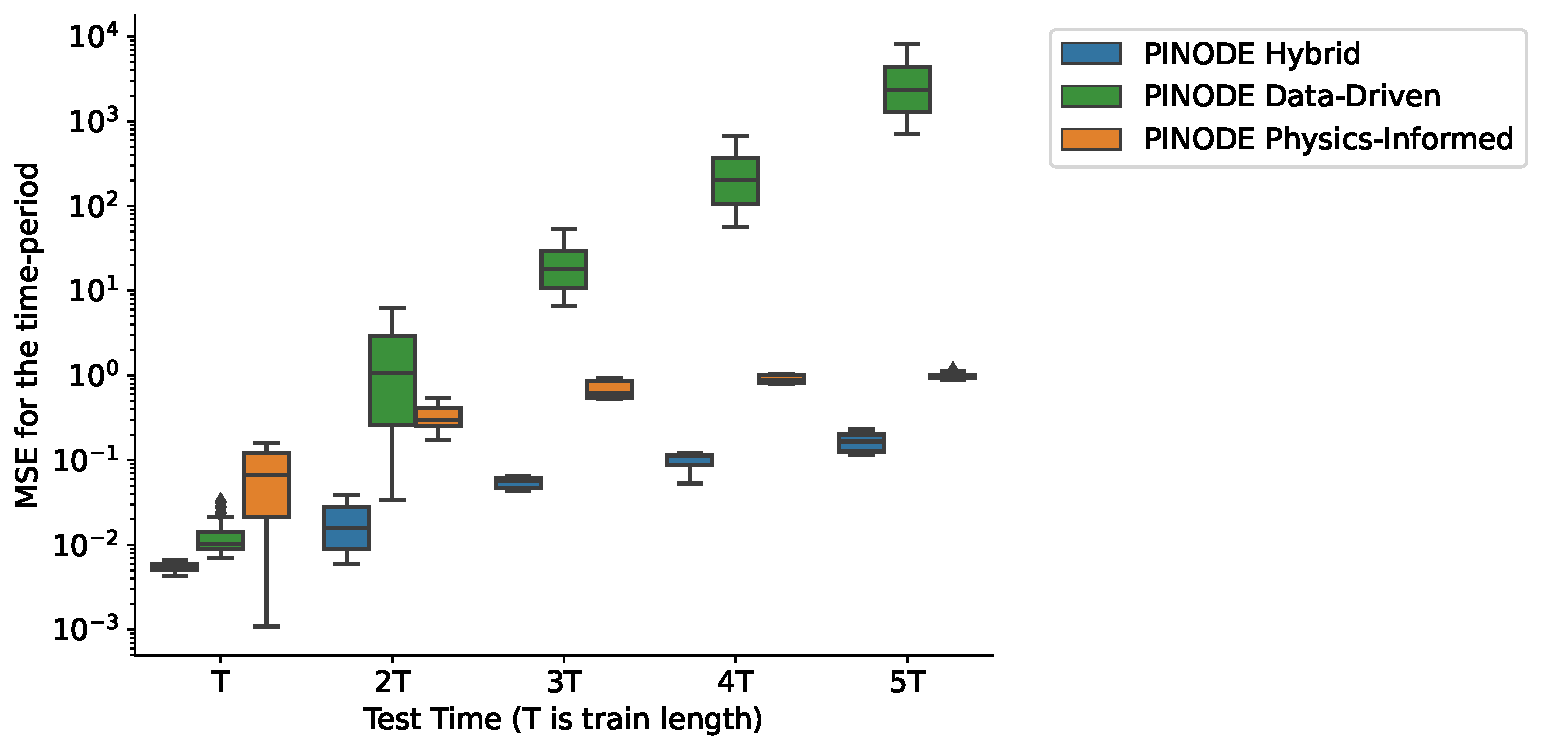
\includegraphics[width=0.75\textwidth]{figures/duffing_periods.pdf}
    \caption{ The time is measured in numbers of training time periods, i.e. $x=3T$ refers the time-range between two and three training time-periods away. The errors of a purely data-driven model grow exponentially when forecasting multiple times father in time than they were trained to do. In contrast, purely Physics-Informed model starts with worst interpolation accuracy but maintains nearly the same error when forecasting far out. Hybrid model combines the short-term accuracy of Data-Driven model and long-term stability of Physics-Informed model.}%\vspace{-0.4in}
    \label{fig:duffing_periods}
\end{figure}




We make two observations from the results displayed in Figure~\ref{fig:duffing_pinode}. First, a purely data-driven model is unable to extrapolate outside its training region using only the data from that region. This observation is consistent with the conclusions from related works~\cite{gin2021deep} that neural networks interpolate well but struggle with extrapolation tasks. Second, we see that collocations provided enough extra information for the model to predict nearly perfectly in regions from which no trajectories were provided. This observation suggests that one can use collocations to ``cover the gaps'' in data and improve the extrapolation accuracy of the model. 

The non-linearity of the Neural ODE plays a crucial role in modeling the latent dynamics. To illustrate, we train a Hybrid PIKN model~\cite{liu2022physics} using the same dataset. PIKN differs from PINODE in using a linear latent dynamics $\frac{dz}{dt} = Lz$, where $L$ is a finite-dimensional approximation of Koopman operator, instead of a general non-linear dynamics $\frac{dz}{dt} = h_\theta(z)$. For PIKN we set $z \in \mathbb{R}^{16}$, an 8 times expansion of the dimension of the true manifold. In Figure~(\ref{fig:duffing_comparison}) we see that PIKN is unable to extrapolate the dynamics to unseen areas correctly using collocations: eventually, all trajectories "collapse" onto the same attractor. DMD shows even worse performance which could be attributed to the linear model reduction.

In the next experiment we show that collocations stabilize long-term predictions of the model even when data from all parts of space is available. To illustrate it we generate a dataset of 6144 trajectories (2048 per red, green, and blue area each) and 50000 collocations uniformly distributed among all three lobes. Next, we train three models: Data-Driven, Physics-Informed, and Hybrid versions of PINODE. Finally, we evaluate their relative performance for ever-increasing forecast time. In Figure~(\ref{fig:duffing_periods}), the x-axis represents test time-period. For example, $x = 2T$ represents prediction errors on a time-period $[2T, 3T)$ where the model was trained on trajectories of length $T$, and on $y$-axis we plot the distribution of prediction errors for 300 unseen trajectories within that period $[2T, 3T)$.

The results on Figure~(\ref{fig:duffing_periods}) show that the performance of the Data-Driven model degrades quickly when the forecasting time-period increases despite an excellent performance when forecasting within its train time-period. Physics-Informed model starts with modest performance but this performance does not degrade when forecasting far ahead. The Hybrid model, in its turn, combines both near-term accuracy with long-term stability, yielding best results over each time period. 

\subsection{Burger's equation}
\label{sec:burger_eqn}
We now study the performance of our framework on Burger's equation with $[-\pi, \pi]$-periodic boundary conditions:
\begin{equation}
\begin{split}
\label{eq:burgers_equation}
    & u_t  + uu_x = \nu u_{xx} \\
    & u(-\pi, t) = u(\pi, t),\quad \forall t \in [0, T]
\end{split}
\end{equation}
where $u_t$, $u_x$, and $u_{xx}$ represent partial derivatives in time, the first, and second spatial derivatives, respectively. Burgers' equation is a PDE occurring in applications to acoustics, gas and fluid dynamics, and traffic flows \cite{burgers1948mathematical}. When $\nu$ is significantly smaller than one, the system exhibits strong non-linear behaviour and is called ``advection-dominated'', otherwise when $\nu$ is large the system is called ``diffusion-dominated''. 
In the case of the former, linear projection methods such as POD become inaccurate as the true solution space has a slow decaying Kolmogorov n-width, manifesting itself in slow decaying singular values \cite{peherstorfer2022breaking}. Therefore, in this section we focus on the advection-dominated Burger for which we set $\nu = 0.01$.


To generate trajectories, we discretize the spacial domain $[-\pi,\,\pi]$ with 128 grid-points, and we solve Equation~\ref{eq:burgers_equation} for $t \in [0, 2]$ with $\Delta t = 0.1$ using a spectral solver~\cite{trefethen2000spectral}. To generate a diverse set of initial conditions we sum the first 10 harmonic terms with random coefficients:
\begin{equation}
    \label{eq:burger_initial_condition}
    u(x, 0) = \frac{1}{10}\sum_{k = 1}^{10} a_k\cos(kx) + b_k\sin((k+1)x), \quad a_k, b_k \sim \mathcal{N}(0, 1)
\end{equation}

To generate collocations we use the same family of functions as we used for the initial conditions in Equation~(\ref{eq:burger_initial_condition}), and we additionally randomize the presence of individual frequencies in the sum:
\begin{equation}
    \label{eq:burger_collocations}
    \bar{u}(x) = \frac{1}{10}\sum_{k = 1}^{10} p_ka_k\cos(kx) + q_kb_k\sin((k+1)x), \quad a_k, b_k \sim \mathcal{N}(0, 1), \quad p_k, q_k \sim Be(1/2).
\end{equation}
We choose this family of collocations to meet the conditions~(\ref{sec:collocations_conditions}). First, this family is representative of the state space $\XX\times Im_f(\XX)$ in the region of interest (moving wave-fronts). Second, (\ref{eq:burger_collocations})~is a smooth set of functions that does not contain unattainable states. Finally, and more importantly, the values $u_x$ and $u_{xx}$ and, consequently $u_t$ can be computed analytically, which makes it especially cheap to sample large amounts of collocations. 

\subsubsection{Compressibility of the Latent Space}

\begin{figure}
    \centering
    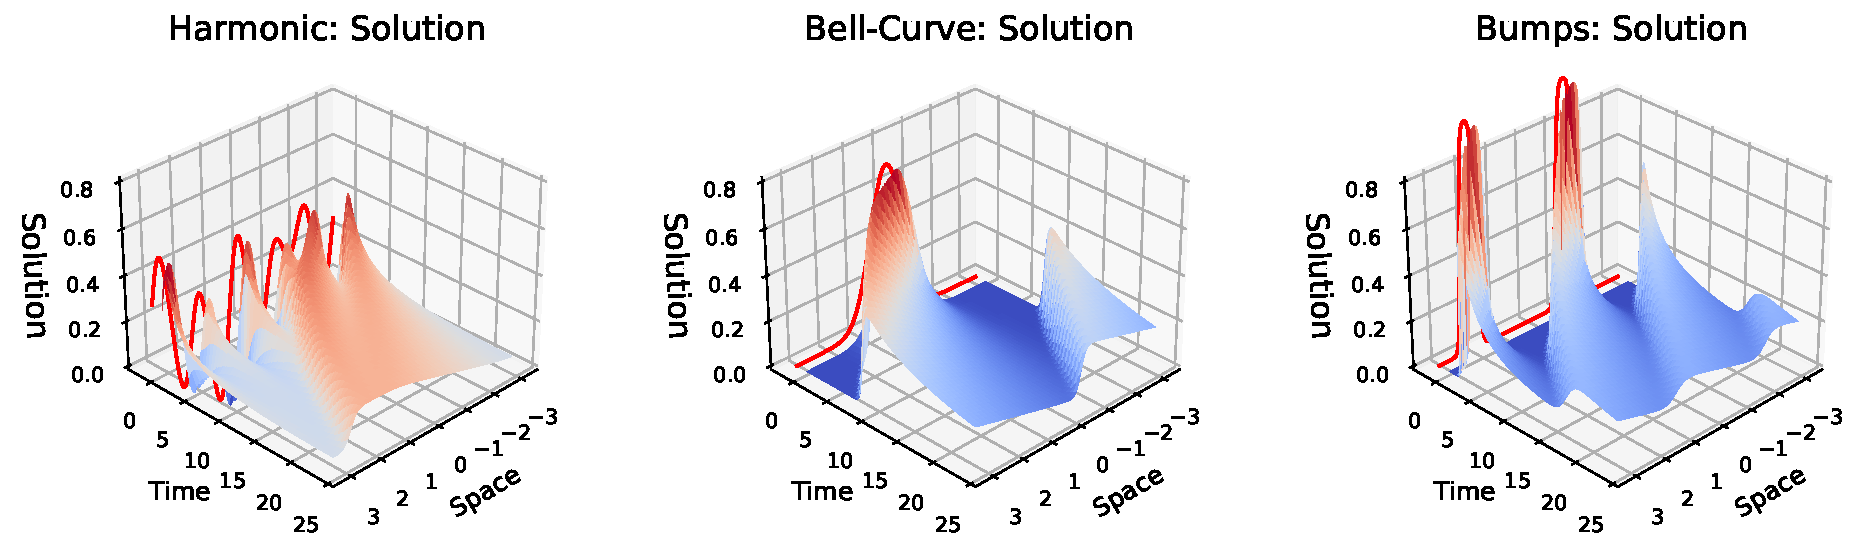
\includegraphics[width=\textwidth]{figures/burgers_examples_of_ics.pdf}
    \caption{Examples of "harmonic", "bell-curve", and "bump" initial conditions, as well as the resulting solutions, in columns 1, 2, and 3 respectively.}
    \label{fig:burgers_examples_of_ics}
\end{figure}

\label{sec:compressibility}
\begin{figure}[t]
    \centering
    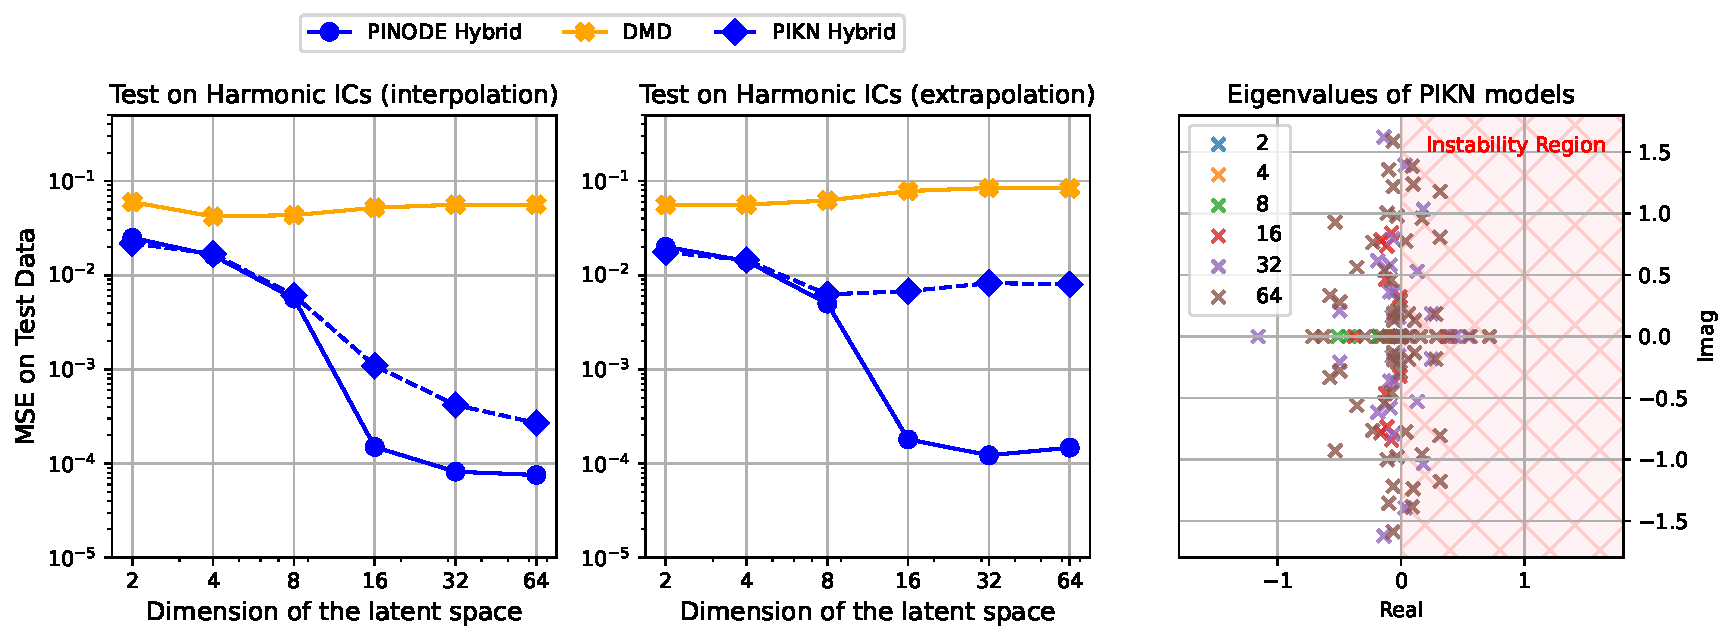
\includegraphics[width=0.9\textwidth]{figures/compressibility.pdf}
    \caption{PINODE Hybrid model utilized the latent space dimension 5 times more efficiently by MSE than PIKN Hybrid model when modelling low-viscosity (highly-nonlinear) Burger's equation (left frame). The difference in performance grows to x100, when forecasting two times farther than the train period (central frame). The reason behind PIKN's long-term instability is the precsence of eigenvalues with poitive real part in the latent dynamics matrix (right frame).}
    \label{fig:burgers_compressibility}
\end{figure}

In Section~\ref{sec:duffing} we showed that a non-linear finite-dimensional latent dynamics model can be a necessity for building a compact ROM for a high-dimensional system. It is \textit{not} the case for Burgers' equations since there is Cole-Hopf transformation that linearize the dynamics. However, a latent-space non-linearity can, in principle, be utilized for finding a more compact latent space, or for increasing the forecast accuracy for the same size of the latent space. In this section we give an example of how PINODE achieves both goals. 

For this experiment we generate 16384 trajectories as described in~(\ref{eq:burger_initial_condition}). We also generate 100000 collocations as described in~(\ref{eq:burger_collocations}). We use the exceedingly large amount of data to allow the models to achieve the best performance for the allowed dimension of the latent space. We evaluate the performance of the models on test data with two different time-frames: (1) same as the training data (\textit{interpolation}), and (2) two times longer than training data (\textit{extrapolation}). More details of the experimental setup are provided in Appendix~(\ref{appendix:burgers_compressibility}).

We compare the performance of three models: DMD, PIKN Hybrid, and PINODE Hybrid. First, we notice that DMD, despite achieving small loss values on training data ($\sim 10^{-3}$), does not perform well on test data. This observation is consistent with earlier works~(\cite{kalur2021robust,kutz2016dynamic}); it illustrates well that a combination of a linear encoder and a linear latent dynamics may not be sufficient for modelling highly-nonlinear phenonmena. Second, we notice that PINODE achieves better performance within a given latent space budget. For instance, for $m = 16$ (Figure~(\ref{fig:burgers_compressibility}), left pane), PINODE achieves $\sim 5$ times lower mean squared error than PIKN, which achieves the same performance only when $m = 512$. More importantly, PINODE maintains low error when predicting for a longer-term horizon (extrapolation in time), which is not the case for PIKN (Figure~(\ref{fig:burgers_compressibility}, right pane). This is a consequence of the latent-dynamics matrix ($h(z) = Lz$) of PIKN having eigenvalues with positive real parts, which implies long-term instability (Figure~(\ref{fig:burgers_compressibility}), right pane). Although there has been progress in the literature~\cite{kojimalearning}, further research is needed to understand (i) how to enforce stability constraints for PIKN, and (ii) why one does not need the same enforcement for PINODE to exhibit stable behaviour. 

\subsection{Training in Low-Data Regime with Collocations}
\label{sec:data_vs_collocations}

\begin{figure}
    \centering
    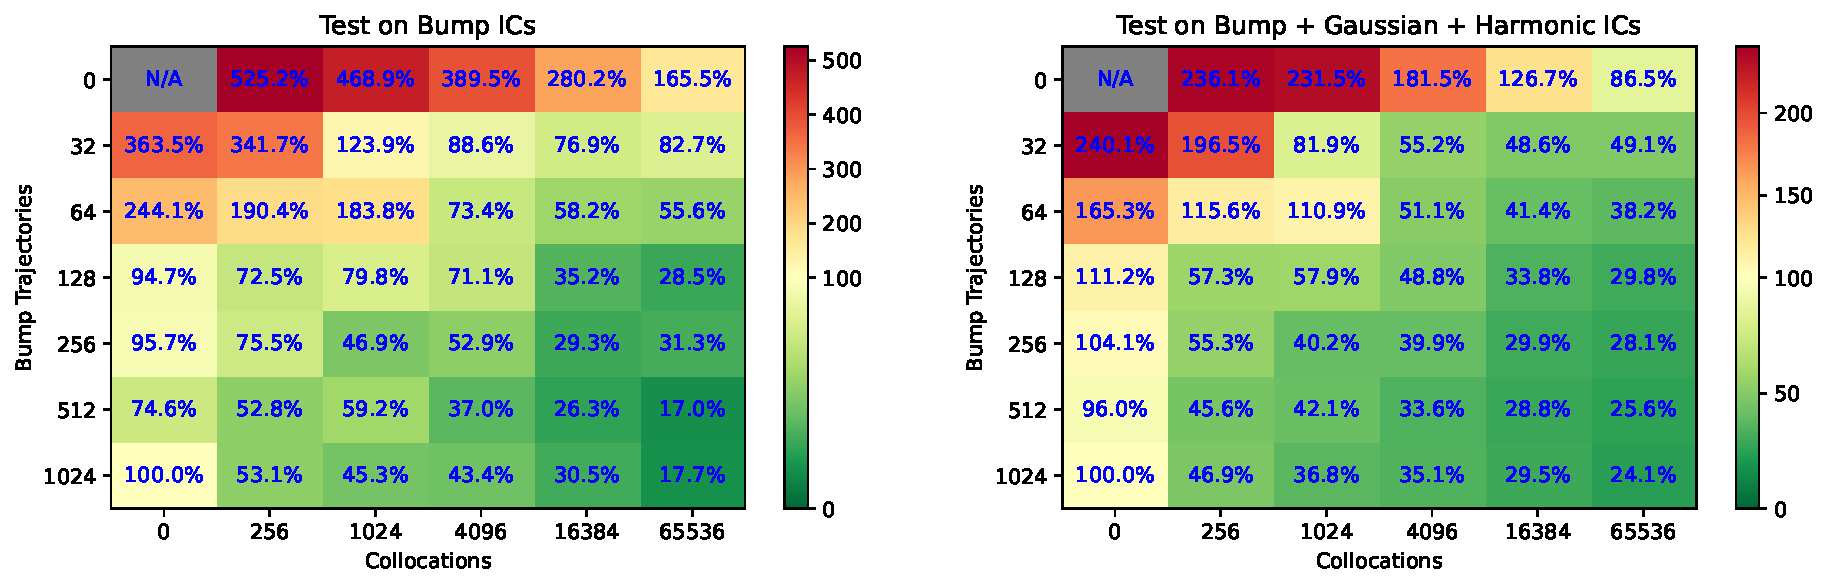
\includegraphics[width=\textwidth]{figures/data_vs_collocations.pdf}
    \caption{The figure shows a comparison of the achievable MSE relative to the full data regime (1024 trajectories). When the data is scarce, collocations-based physics-informed loss improves the forecasting accuracy of ROMs by an average of 5 times lower MSE compared to the data-only regime, as shown in this experiment with Burger's equation. Moreover, when other types of initial conditions (``harmonic'', ``bell-curve'') are used, the physics-only model (top-right corner of the right frame) outperformed the most data-rich model in our experiment (bottom-left corner). }
    \label{fig:burger_data_vs_collocations}
\end{figure}

In the next experiment we study relative efficiency of using collocations against using data in a low-data regime. It is frequently the case that only a small number of simulations (or measurements) can be obtained for a physical system of interest due to the computational, time, or budget constraints. We would like to compensate the lack of data with providing collocations which are considerably cheaper to generate. The collocations, however, can be a ``weaker'' signal for the model than real data, especially when time passes and the shape of the solution moves out of the collocation family's span. In this section we show that collocations can be effectively used for this goal, when chosen right, and their contribution to a model's accuracy may even surpass the contribution of the data. 




\begin{figure}
    \centering
    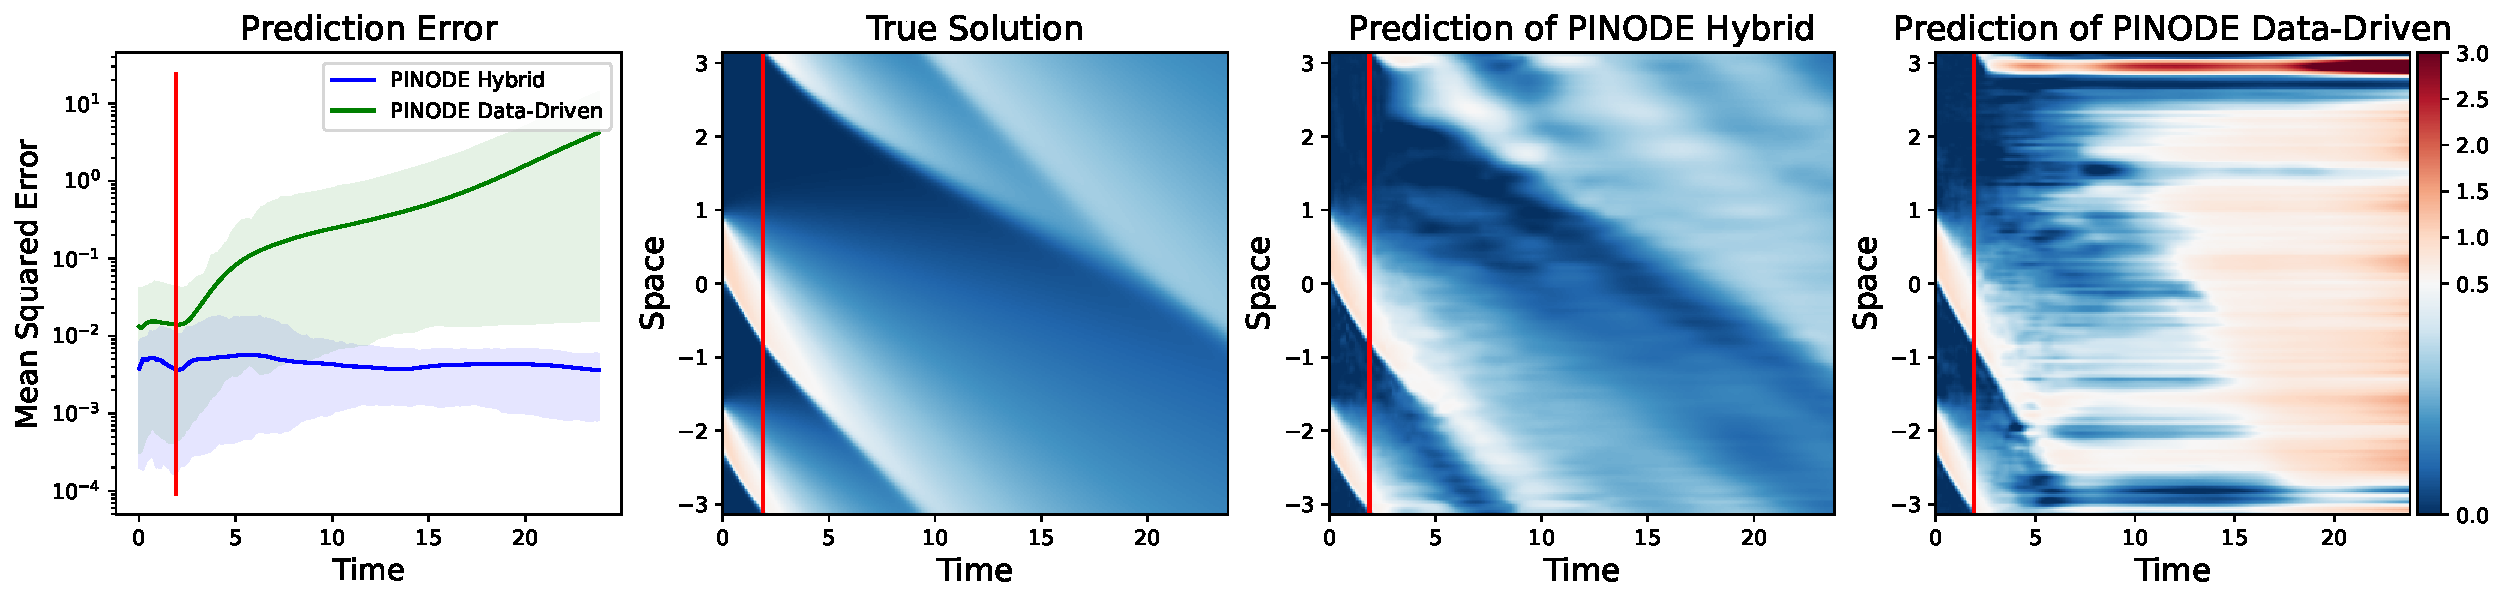
\includegraphics[width=\textwidth]{figures/example_burgers.pdf}
    \caption{The first subplot shows the relative error of solving Burger's equations on 100 test (unseen) initial conditions for two models: PINODE Hybrid and PINODE Data-Driven. Both models interpolate well but a purely data-driven model fails to extrapolate past the time-period that it was trained on (to the left of the red line). PINODE-Hybrid provides stable long-term predictions that indicates a high-quality of a discovered low-dimensional manifold dynamics. An example of such effect is provided on subplots~2-4.}
    \label{fig:burgers_example}
\end{figure}

To illustrate the trade-off between data and collocations, we train one model per various combinations of number of trajectories vs collocations in their training sets. To gauge the extrapolation power of our models, we use trajectories with three types of initial conditions: ``harmonic'', ``bell-curve'', and ``bumps'' (see Figure~(\ref{fig:burgers_examples_of_ics}) for equations and illustrations). For training, we use 2048 trajectories with ``bumps'' initial conditions. For collocations, we use the harmonic family as described in~(\ref{eq:burger_collocations}). We use two test datasets: (1) 100 trajectories with ``bump'' ICs to assess within-distributuion performance, left frame), and (2) a mix of trajectories with ``bump'', ``bell-curve'', and ``harmonic'' initial conditions, 100 of each, to assess out-of-distribution performance. All test data trajectories were two times longer than the train trajectories. More details on the experimental setup are provided in Appendix~\ref{appendix:burgers_data_vs_collocations}. We fit one PINODE model with the latent dimension $m = 16$ per each combination of the amount of data and collocations. On Figure~(\ref{fig:burger_data_vs_collocations}) we report its performance on two test datasets relative to the richest data-driven model with no collocations (bottom-left corner). 

From the results displayed on Figure~(\ref{fig:burger_data_vs_collocations}) we see that adding collocations always improved the model in our experiments.  Moreover, when a sufficient number of collocations is added in training, the model with fewer data snapshots was always able to outperform the model with the maximum amount of data but no collocations. On average, a collocation-aided model was \textit{5 times better} at both within-distribution and out-of-distribution performance relative to a purely data-driven version of the model. In addition, we noticed that a model that used only collocations can perform better than a data-rich model, especially when predicting the dynamics of the unseen initial conditions (Figure~(\ref{fig:burger_data_vs_collocations}), right pane, top-right vs bottom-left corner). 

We also notice that the Hybrid models yield more stable and accurate predictions, relative to their purely data-driven counterparts, when forecasting far beyond the training time-period. In Figure~(\ref{fig:burgers_example}) we visualize the predictions for a test IC for two models: Data-Driven model from the bottom-left corner of Figure~(\ref{fig:burger_data_vs_collocations}), and a Hybrid model from the bottom-right corner of Figure~(\ref{fig:burger_data_vs_collocations}). The red line separates the time-period of training from the time-period of forecasting. The hybrid model's errors stay below $10^{-2}$ even when forecasting 10 times farther than what it was trained on. In contrast, Data-Driven model shows similarly low errors within its training time-region but the forecast errors grow quickly when forecasting beyond that.

\subsection{Robustness to Noise in Low-Data Regime}
\label{sec:burger_noise}
\begin{figure}[t]
    \centering
    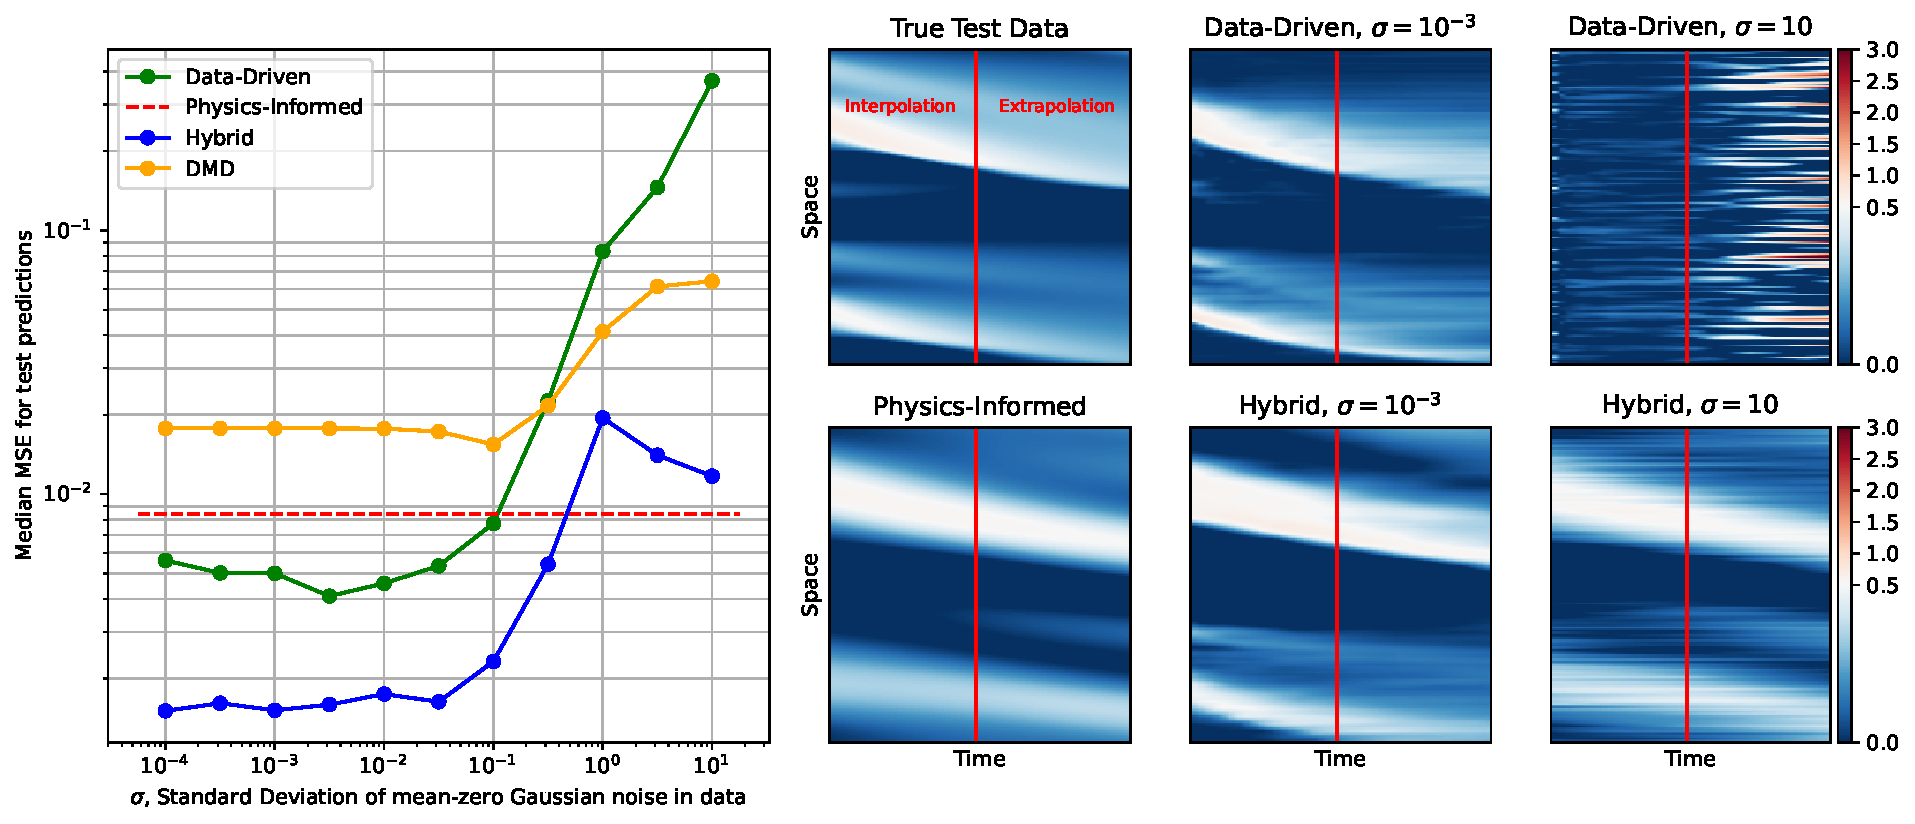
\includegraphics[width=\textwidth]{figures/burgers_noise.pdf}
    \caption{Physics-informed loss works as a safeguard that prevents unbounded performance drop when quality of the data degrades due to noise. Namely, the solution of the hybrid loss~(\ref{eq:loss_combined}) converges to the solution of the physics-informed loss~(\ref{eq:loss_physics_informed}), when the data-driven loss~(\ref{eq:loss_physics_informed}) becomes uninformative. The performance of purely data-driven methods (Data-Driven, DMD) grows unbounded since these models don't have an alternative noise-independent source of information.}
    \label{fig:burger_noise}
\end{figure}

In this section we show that the use of collocations improves the ROM's robustness when the data is noisy by providing an alternative, noise-free, source of information.

For this experiment, we use the datasets from the bottom-right cell of Figure~(\ref{fig:burger_data_vs_collocations}), Pane~2. Namely, we use 1024 trajectories with "bump" initial conditions (an example is on Figure~(\ref{fig:burgers_examples_of_ics})), and we use 65536 "harmonic" collocations as defined in Equation~\ref{eq:burger_collocations}. We then add i.i.d. Gaussian noise to the trajectories, with the variance ranging from $\sigma = 10^{-4}$ to $\sigma = 10$. For reference, most of the data values lie between $0$ and $1$, so a noise level with $\sigma > 1$ dominates the data. We train four models: PINODE Hybrid, PINODE Data-Driven, PINODE Physics-Informed, and DMD. To measure the models' out-of-distribution prediction errors we use the Test Dataset 2 from the previous section; this dataset consists of three types of noise-free trajectories (see Figure~\ref{fig:burgers_examples_of_ics}), 100 each. The errors are displayed on Figure~(\ref{fig:burger_noise}), left pane. The error of a purely Physics-Informed model (in red) is flat because the collocations are noise-free and thus the same for all noise-levels, so we only train this model once. 

On Figure~(\ref{fig:burger_noise}) we see that, when noise is high, the error of purely data-driven models grows unbounded, whereas the performance of the hybrid method converges to the performance of the Physics-Informed model. We hypothesise that it happens because the second part~($\LL_{\theta}^{data}$) of the combined loss~(Eq.~\ref{eq:loss_combined}) turns into noise, and so its derivative also turns into noise.
\begin{equation}
    \nabla \LL_{\theta} = \underbrace{\nabla\LL_{\theta}^{physics}}_{\text{informative}} + \underbrace{\nabla\LL_{\theta}^{data}}_{\text{noise}}
\end{equation}
Thus, one can think about optimizing a hybrid model~(\ref{eq:loss_combined}) as about training Physics-Informed model~(\ref{eq:loss_physics_informed}) using a noisy gradient descent with a fixed-variance noise. From the optimization literature \cite{friedlander2012hybrid,patel2021global,shapiro2021lectures} we know that, under certain conditions, such SGD converges to a neighbourhood of a local minima of its loss (in this case $\LL_{\theta}^{physics}$) with high probability. So instead of diverging, a hybrid model turns into Physics-Informed model; where the latter works as a performance safeguard in the high-noise regime.  On the right hand-side of Figure~(\ref{fig:burger_noise}) we show an example of the prediction performance of each of the models described above. The data-driven and hybrid models yield visually similar solutions when $\sigma = 10^-3$. However, the former provides inadequate performance when the data is dominated by noise (which is expected), whereas a hybrid model in this regime produces a solution that is visually similar to the one that Physics-Informed model produces. A more rigorous analysis of this phenomenon seems possible but lies outside of the scope of this paper.


\section{Discussion and Conclusions}

In this work we demonstrated how a collocation point technique can improve the performance of an emerging class of continuous-time neural-network based reduced-order models. First, it can ``cover the gaps'' in datasets and inform the model about underrepresented basins of attraction. It alleviates the demand for large volumes of data that is common in network-based models, which is crucial in applications where the data is scarce and expensive. Second, the physics-informed loss may work as a safeguard, providing a noise-independent source of truth.
Third, collocations can stabilize the model's long-term predictions, allowing to accurately forecast far beyond the training horizon. Finally, together with using a NODE-based non-linear latent dynamics, adding physics-informed loss leads to discovery of more compact latent spaces that yield more accurate models. Simultaneous stability and compactness is especially important if one aims to use models together with compressive sensing and control algorithms.

One clear limitation of the current work is that the choice of an efficient collocation family is a design decision that a practitioner makes. The authors believe that such decisions can be automated by adopting existing approaches from classic works on numerical approximations of PDEs, which we leave for future research. Another automation that prompts future research is more efficient way of sampling collocation points, possibly via applying modern adaptive learning techniques \cite{subramanian2022adaptive}. Finally, although Section~\ref{sec:burger_noise} provides some rationale why one may expect robustness of Hybrid models under noise, the authors believe that a more rigorous analysis is possible; particularly one that provides conditions under which such robustness is guaranteed. 